\chapter{Diffusion et reproduction des travaux}
\label{sec:reproductibility}

Dans ce chapitre, nous discutons de la reproduction puis de la diffusion de nos travaux. En effet, un de nos objectifs principaux était la réutilisation de notre travail (filtres, banc de test, etc.) par des tiers souhaitant utiliser ou créer des filtres de rehaussement de vaisseaux. Nos travaux peuvent évidemment s'appliquer au rehaussement d'autres structures présentant des propriétés similaires dans des images 3D.

\section{Reproduction}
\subsection{Définitions}

La reproduction des résultats de recherche est une part aussi importante que leur diffusion, qu'elle peut part ailleur favoriser. Bien que la diffusion soit fermement implantée dans la communauté scientifique par la publication d'articles ou la communication à travers des conférences nationales ou internationales, l'aspect reproduction est plus souvent négligé. Pourtant, celle-ci est primordiale pour la recherche. Elle contribue à rendre transparentes toutes les étapes d'une expérience et d'en révéler les éventuelles erreurs. Elle permet en particulier la validation des résultats par des tiers, qui est la base du consensus scientifique.

Il existe différentes options et concepts liés à la reproduction des résultats. La définition de la reproduction de travaux est en effet variable selon les auteurs. Nous utilisons ainsi les définitions proposées par l'ACM \footnote{\url{https://www.acm.org/publications/policies/artifact-review-and-badging-current}} (\textit{association of computing machinery}) qui présente différents degrés de reproduction. Les auteurs distinguent trois définitions : 

\paragraph{La répétabilité (même équipe - même équipement)}

La répétabilité consiste à ce qu'une équipe de chercheurs puisse reproduire ses propres expériences de manière consistante avec la même précision, la même méthodologie et le même équipement. Pour les expériences calculatoires, cela signifie qu'un chercheur peut répéter ses propres calculs de manière constante.


\paragraph{La reproductibilité (équipe différente - même équipement)}

La reproductibilité consiste à ce qu'une équipe de chercheurs différente de l'équipe initiale puisse reproduire les résultats de la première équipe avec la même précision et en utilisant la même méthodologie et les mêmes conditions d'opérations. Pour les expériences calculatoires, cela veut dire qu'un chercheur indépendant peut obtenir les mêmes résultats en utilisant la base de code de l'auteur original.

\paragraph{La réplicabilité - (équipe différente - équipement différent)}

La réplicabilité consiste à ce qu'une équipe indépendante puisse reproduire les résultats d'une autre équipe à une précision donnée avec leur propre équipement et leurs propres algorithmes. Pour des expériences calculatoires, cela veut dire qu'un groupe indépendant peut reproduire les mêmes résultats avec sa propre implémentation.

\subsection{Reproductibilité du banc de test}

Pour notre travail, il était évident que notre banc de test devait être reproductible. En effet, c'est la condition minimale à remplir pour qu'un autre utilisateur puisse appliquer et/ou étendre nos travaux. Un autre avantage est qu'un code reproductible sert aussi de base d'exemples pratiques dont l'utilisateur futur peut s'inspirer pour créer ses propres expériences.

Comme présenté dans les Chapitres 3 et 4, le banc de test complet a nécessité 5 éléments : les bases de données, les filtres, le banc de test, les fichiers de paramètres des expériences et enfin les scripts d'analyse des résultats selon un critère d'optimisation.

De manière à ce qu'un utilisateur puisse réutiliser nos données, nous avons rendu publics les volumes des jeux de données modifiés sur un serveur du LIRIS. Cette méthode assure donc la reproductibilité au niveau des données, puisque les mêmes volumes utilisés dans nos expériences peuvent être téléchargés. Cette première solution reste cependant fragile, puisque l'aléa de l'entretien de petites plateformes peut rendre ces données indisponibles. C'est par exemple le cas pour le banc de test de Manh Lu présenté dans le Chap. 3. Nous avons donc proposé une seconde option en rendant disponible le code permettant de générer l'ensemble des masques, des zones d'intérêt et des volumes modifiés à partir des bases de données publiques. Cette seconde option est cependant réplicable et non reproductible puisqu'une partie des artefacts, notamment le bruit est appliqué de manière aléatoire. Elle pourrait devenir reproductible si nous avions conservé les graines initialisant les générateurs de variables aléatoires, ce qui n'est pas le cas.  

L'ensemble du code pour les filtres, le banc de test, les outils de génération des fichiers de paramètres ainsi que les scripts d'analyses est disponible publiquement sur un dépôt de la plateforme GitHub (\url{https://github.com/JonasLamy/LiverVesselness}). Nous avons différencié les versions associées aux publications majeures de nos travaux de manière à garder une traçabilité des itérations de nos travaux et d'associer une base de code à une publication spécifique. On évite ainsi de ne seulement conserver que la version la plus récente et de perdre la reproductibilité sur les publications intermédiaires telles que les articles de conférence.

Nous avons aussi rendu public les fichiers de paramètres permettant de lancer l'ensemble des calculs du banc de test. Ces fichiers sont répartis en trois catégories~: 

\begin{itemize}
\item Les fichiers de configuration du banc de test pour le calcul de métriques ;
\item les fichiers de description des bases de données ;
\item les fichiers listant les paramètres des filtres.  
\end{itemize}

L'usage de ces fichiers rend la reproduction du calcul des métriques transparente, puisque l'ensemble du paramétrage est déjà effectué pour les 60 sous-parties de l'analyse (7 filtres, 2 étapes d'optimisation sauf RORPO et Meijering, 5 bases de données).

Ce système de paramétrage a été mis à l'épreuve avec succès lorsque nous n'avions pas de cluster de calcul à disposition et que nous devions déployer le banc de test sur plusieurs machines différentes. Le banc de test a été utilisé sur deux types de systèmes d'exploitation différents, à savoir Linux et Mac OS.

\begin{table}[!t]
    \resizebox{\textwidth}{!}{
    \begin{tabular}{lcccc}
        
    \hline
    Étape                               & Répétable  & Reproductible   & Réplicable & Automatisation totale  \\
    Génération des jeux de paramètres   &     X      &       X         &     X      &          -           \\
    Génération des volumes              &     X      &       X         &     *      &          X           \\
    Calcul des métriques                &     X      &       X         &     *      &          X           \\
    Calcul des paramètres optimaux      &     X      &       X         &     *      &          -           \\
    \hline
    \end{tabular}
    }
    \caption{ Tableau récapitulant les propriétés de notre banc de test. Bien que reproductibles, certaines étapes nécessitent une modification manuelle en fonction des bases de données. Les * signifient que les résultats sont répétables dans le cas où l'on définit à l'avance les graines des générateurs aléatoires }
    \label{ tab:reproductibility }
\end{table}

\subsection{Stabilité des calculs} 

La réplicabilité est difficile à obtenir sur ce genre de banc de test, relativement complexe. En effet, la diversité des OS et le type d'encodage des valeurs numériques, aussi bien pour les données que pour le banc de test sont susceptible de faire varier les résultats. Pour assurer la réplicabilité, il faudrait ainsi s'assurer, architecture par architecture, de la stabilité des calculs. Par exemple, l'encodage des types primitifs (\textit{int}, \textit{float}, \textit{double}), et donc leur précision peuvent varier selon les machines. Sur certaines opérations, et notamment en travaillant avec des nombres flottants, une perte de précision peut avoir lieu. Sur des calculs cumulatifs, celle-ci peut devenir significative.

Nous n'avons pas assuré la réplicabilité de notre banc de test. Cependant, nous avons essayé de limiter au maximum les instabilités de notre code. Par exemple, nous avons détecté puis corrigé des inconsistances dans le seuillage des volumes de sortie après filtrage. En effet, notre test de binarisation pouvait générer une classification inconsistante des voxels suivant la représentation des nombres flottants générés. Typiquement un test d’infériorité au sens large (Eq. \ref{eq:test_1}) pouvait être erroné si aucune valeur d’approximation n'était utilisée (par ex 0.6 représenté par 0.59999999).

\begin{align}
    p(x) &=
    \begin{cases}
        1, \text{si} I(x) \leq \text{seuil} \\
        0, \text{sinon}
    \end{cases}
    \label{eq:test_1}
\end{align}
 
Le calcul des métriques étant réalisé par cumul des valeurs des matrices de confusion à chaque seuil, on obtenait alors un décalage important entre l'algorithme naïf de seuillage et celui effectué et discuté dans le chapitre 3. La réécriture de ce test en incluant un epsilon basé sur le nombre de chiffres significatifs du seuil permet de résoudre cette inconsistance (Eq. \ref{eq:test_2}).
 
 \begin{align}
    p(x) &=
    \begin{cases}
        1, \text{si} I(x) \leq (\text{seuil} - \epsilon) \\
        0, \text{sinon}
    \end{cases}
    \label{eq:test_2}
\end{align}
 
 Avec $\epsilon = \frac{1}{ \text{Nb seuils} } 1\exp^{-3}$.

Enfin, il est important de noter qu'il est difficile de réaliser des travaux reproductibles et réplicables de manière solitaire. En effet, tester soit même ses outils a ses limites, en particulier des erreurs peuvent passer inaperçues par effet d'accoutumance lié à la lecture d'un code familier. Il est donc indispensable que des personnes extérieures puissent proposer un retour d'expérience sur ce type de projets.

\subsection{Temps}

Un autre argument en faveur d'un code ouvert et reproductible est l'aspect lié au temps de calcul et aux ressources disponibles. Bien que notre banc de test n'inclut pas lui-même de statistiques sur le temps de calcul, nous avons pu mesurer ces valeurs grâce au cluster de l'IN2P3 (Institut national de physique nucléaire et de physique des particules) sur lequel nous avons lancé nos expériences pour la deuxième itération de nos travaux. 

Sur un cluster, le temps de calcul se différencie entre le temps horloge (\textit{Wallclock time}) et le temps CPU (\textit{CPU time}). Dans le premier cas, le temps horloge correspond au temps passé par l'ensemble du processus. Le temps CPU ne renseigne que le temps d'utilisation du CPU et ne prend donc pas en compte les appels systèmes ou les écritures/lectures sur le disque. Sur un cluster, les temps de calcul sont estimés en unité HS06.h\footnote{\url{https://w3.hepix.org/benchmarking.html}}. La norme HS06 est une norme pour banc de test qui permet de mesurer pour une quantité d'énergie, la quantité de travail réalisé par un système. L'unité HS06.h est donc une unité d'heure définie dans le contexte de ce banc de test. Le temps CPU est aussi exprimé de manière linéaire et non de manière parallélisée. Cela veut dire qu'un calcul de deux heures parallélisé en 3 processus correspond à 6h de \textit{Wallclock time}. L'ensemble du temps de calcul nécessaire à la réalisation des résultats présentés dans le Chap. 4 est récapitulé dans la Tab. \ref{tab:consumption_in2p3}.

\begin{table}
    \centering
    \begin{tabular}{lcc}
        \hline
        Temps         & HS06.h   & Temps réel \\
        Horloge       &  178 521 &    11 157  \\
        CPU           &  83 348  &     5 209  \\
    \end{tabular}
    \caption{Consommation en heures de calculs des ressources de l'IN2P3 pour produire les résultats pour la dernière itération de nos travaux (essais préliminaires, erreurs de lancement et banc de test compris). Pour l'IN2P3, le temps réel est estimé en divisant par 16 le temps HS06.h}
    \label{tab:consumption_in2p3}
\end{table}


\section{Diffusion}

\subsection{Communication scientifique}
Nous avons présenté notre travail dans différentes conférences et journaux scientifiques. Lors de la création du banc de test, une première communication sans acte a eu lieu à VPH 2020 (Virtual Physiological Human) à Paris \cite{Lamy2020_VPH_bench}. Une première analyse des filtres de rehaussement avec la première itération de l'optimisation des paramètres des filtres a été présentée à ICPR 2020 (International Conference on Pattern Recognition) \cite{Lamy2020_ICPR} ainsi que le fonctionnement du banc de test en tant qu'article complémentaire au workshop RRPR (Reproducible Research in Pattern Recognition) \cite{Lamy2021_RRPR}. Ces travaux ont aussi été présentés à la  conférence nationale ORASIS 2021 à Toulouse \cite{Lamy2021_ORASIS}. Enfin la seconde itération du banc de test, incluant la deuxième version de l'optimisation, l'analyse du rehaussement en fonction de la taille des vaisseaux et l'ajout de la base Bullitt a été publiée dans le Journal IEEE Transactions on Medical Imaging \cite{Lamy2022_TMI}.

Ces travaux sont accompagnés d'un dépôt GitHub où l'on peut retrouver l'ensemble du code : \url{https://github.com/JonasLamy/LiverVesselness}. 


\subsection{Démonstration en ligne}

Le choix de découpler l'implémentation du banc de test des CLI formés par les filtres de rehaussement nous a permis de mettre en place une démonstration en ligne. Elle permet de tester les 7 filtres de rehaussement utilisés dans nos travaux sans aucune installation préalable. L'utilisateur peut sélectionner un filtre et régler ses paramètres intrinsèques ainsi que l'échelle de détection des vaisseaux afin d'observer le comportement et la stabilité du rehaussement. Dans cette démonstration, l'utilisateur peut choisir d'appliquer les filtres dans des zones d'intérêt particulières selon le même principe utilisé dans le banc de test. Un ensemble de volumes de test issus de l'Ircad et de VascuSynth ainsi qu'un ensemble de masques tels que le foie, le voisinage des vaisseaux et les bifurcations sont sélectionnables. De plus l'interface utilisateur permet de téléverser ses propres volumes sur lesquels il est possible d’appliquer les différents filtres. Là aussi, l'utilisateur peut choisir d'utiliser ses propres zones d'intérêt. Tous les types d'images volumiques supportés par la librairie ITK peuvent être utilisés tel que le \textit{.vol}, \textit{.nii}, \textit{.nii.gz}, \textit{.mhd}, ou \textit{.mha} avec une taille inférieure à 50 Mo.

\begin{figure}[!ht]
    \begin{subfigure}{0.45\textwidth}
        \centering
        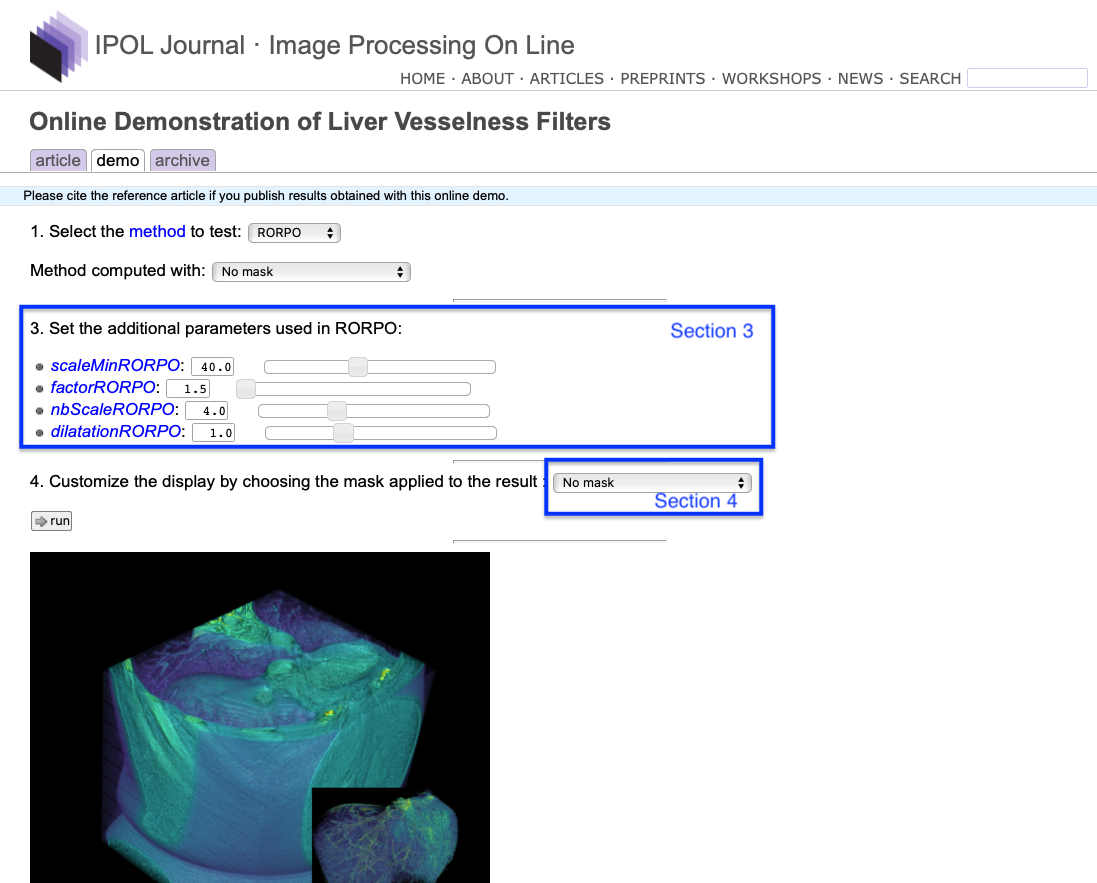
\includegraphics[width=8cm]{Images/visuBenchmarkDemos.png}
        \caption{Paramétrisation}
    \end{subfigure}
    \begin{subfigure}{0.45\textwidth}
        \centering
        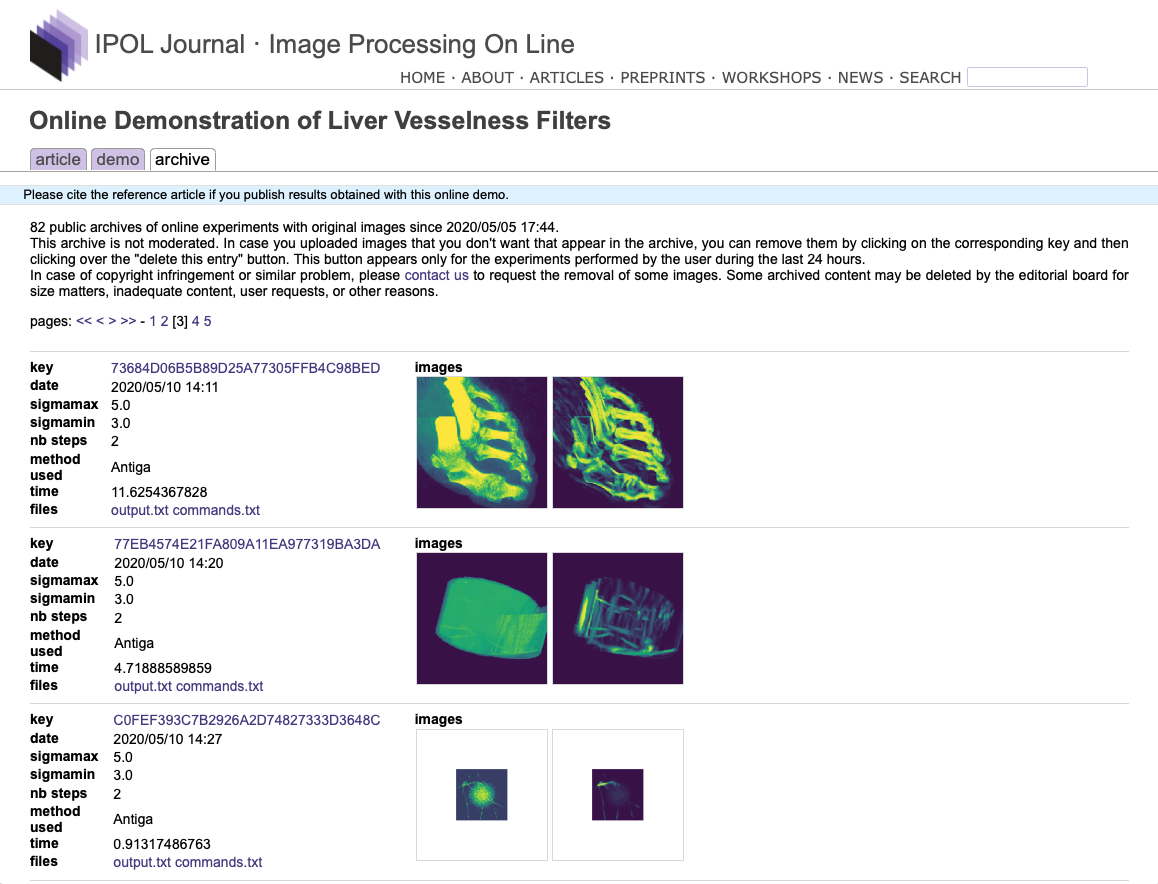
\includegraphics[width=8cm]{Images/visuBenchmarkDemosArchivesTrim.png}
        \caption{Historique}
    \end{subfigure}

    \caption{Illustration de l'interface de la démonstration en ligne. (a) Interface principale permettant de choisir les paramètres d'échelles et les paramètres intrinsèques, ainsi que les masques d'images (encadrés en bleu). (b) Section d'historique des images testés par les utilisateurs anonymes.}
\label{Fig:DemoExample}
\end{figure}

La démonstration propose un résultat sous forme de visualisation 3D du rehaussement. Le visualisateur 3D utilisé pour cette démonstration est \textit{itk-vtk-viewer}~\cite{Mccormick2020_Visu3DDemo}. Il propose la visualisation du volume résultat avec une superposition de la vérité terrain (quand celle-ci est disponible). Le viewer permet aussi d'ajuster la fenêtre d'intensité et le contraste de la visualisation des filtres. Il permet également la vue de coupes 2D.

La démonstration est disponible sur le site du journal IPOL (Image Processing On Line)\footnote{\url{ https://kerautret.github.io/LiverVesselnessIPOLDemo/}}.

\begin{figure}[!t]
\noindent   
\centering
    \begin{subfigure}{0.33\textwidth}
        \centering
        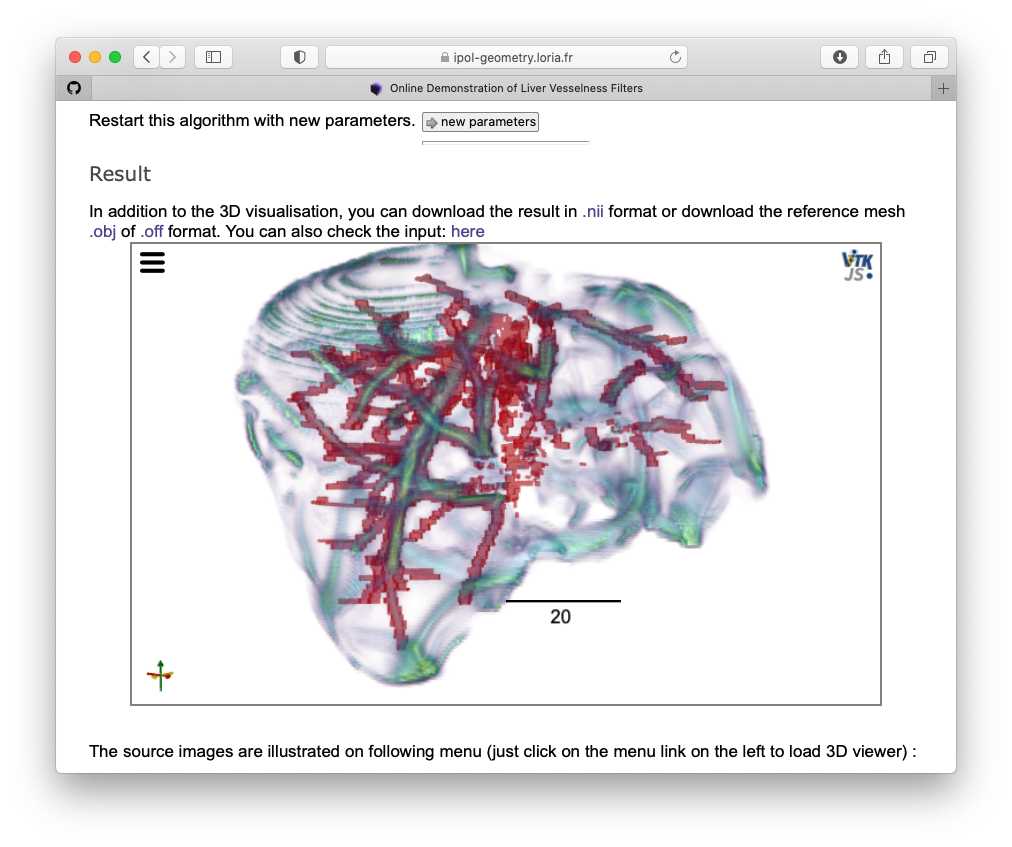
\includegraphics[width=5cm, trim= 4.7cm 5cm 4.7cm 8.5cm, clip=true]{Images/visuDemoViewer.png}
        \caption{ }
    \end{subfigure}
    \begin{subfigure}{0.33\textwidth}
        \centering
        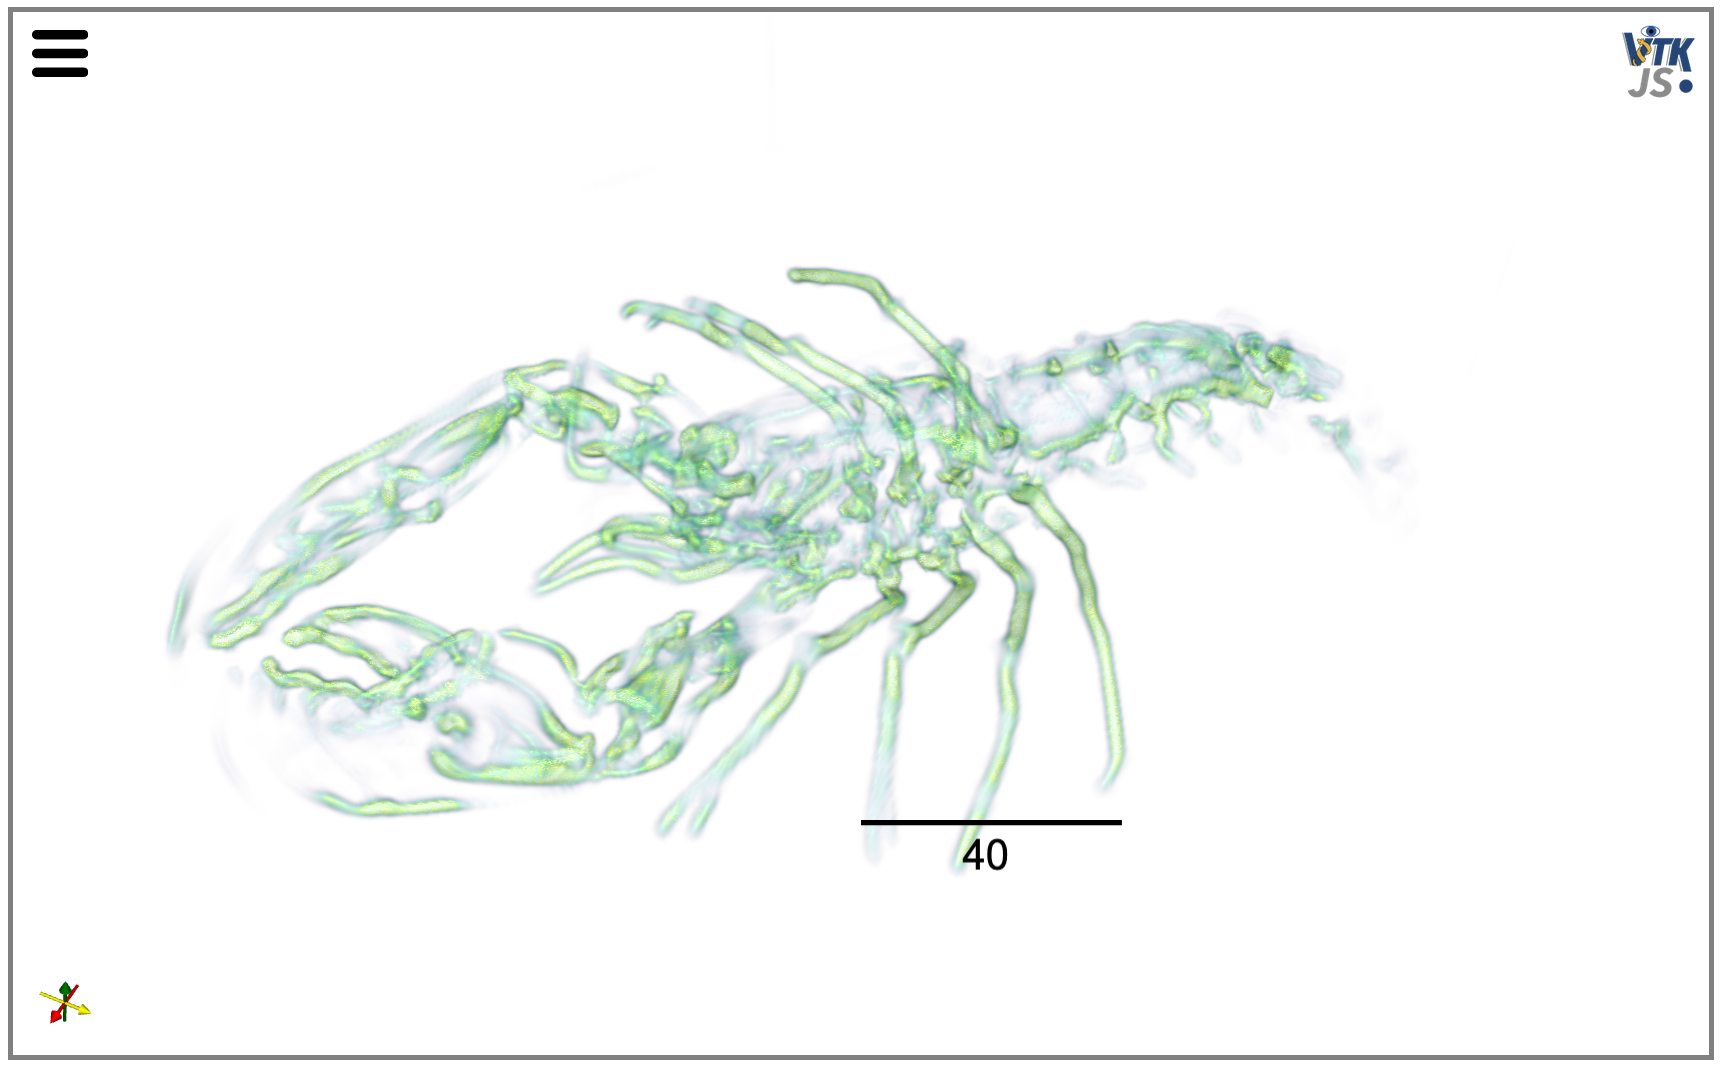
\includegraphics[width=5cm]{Images/visuDemoViewerExtract.png}
        \caption{ }
    \end{subfigure}
    \begin{subfigure}{0.33\textwidth}
        \centering
        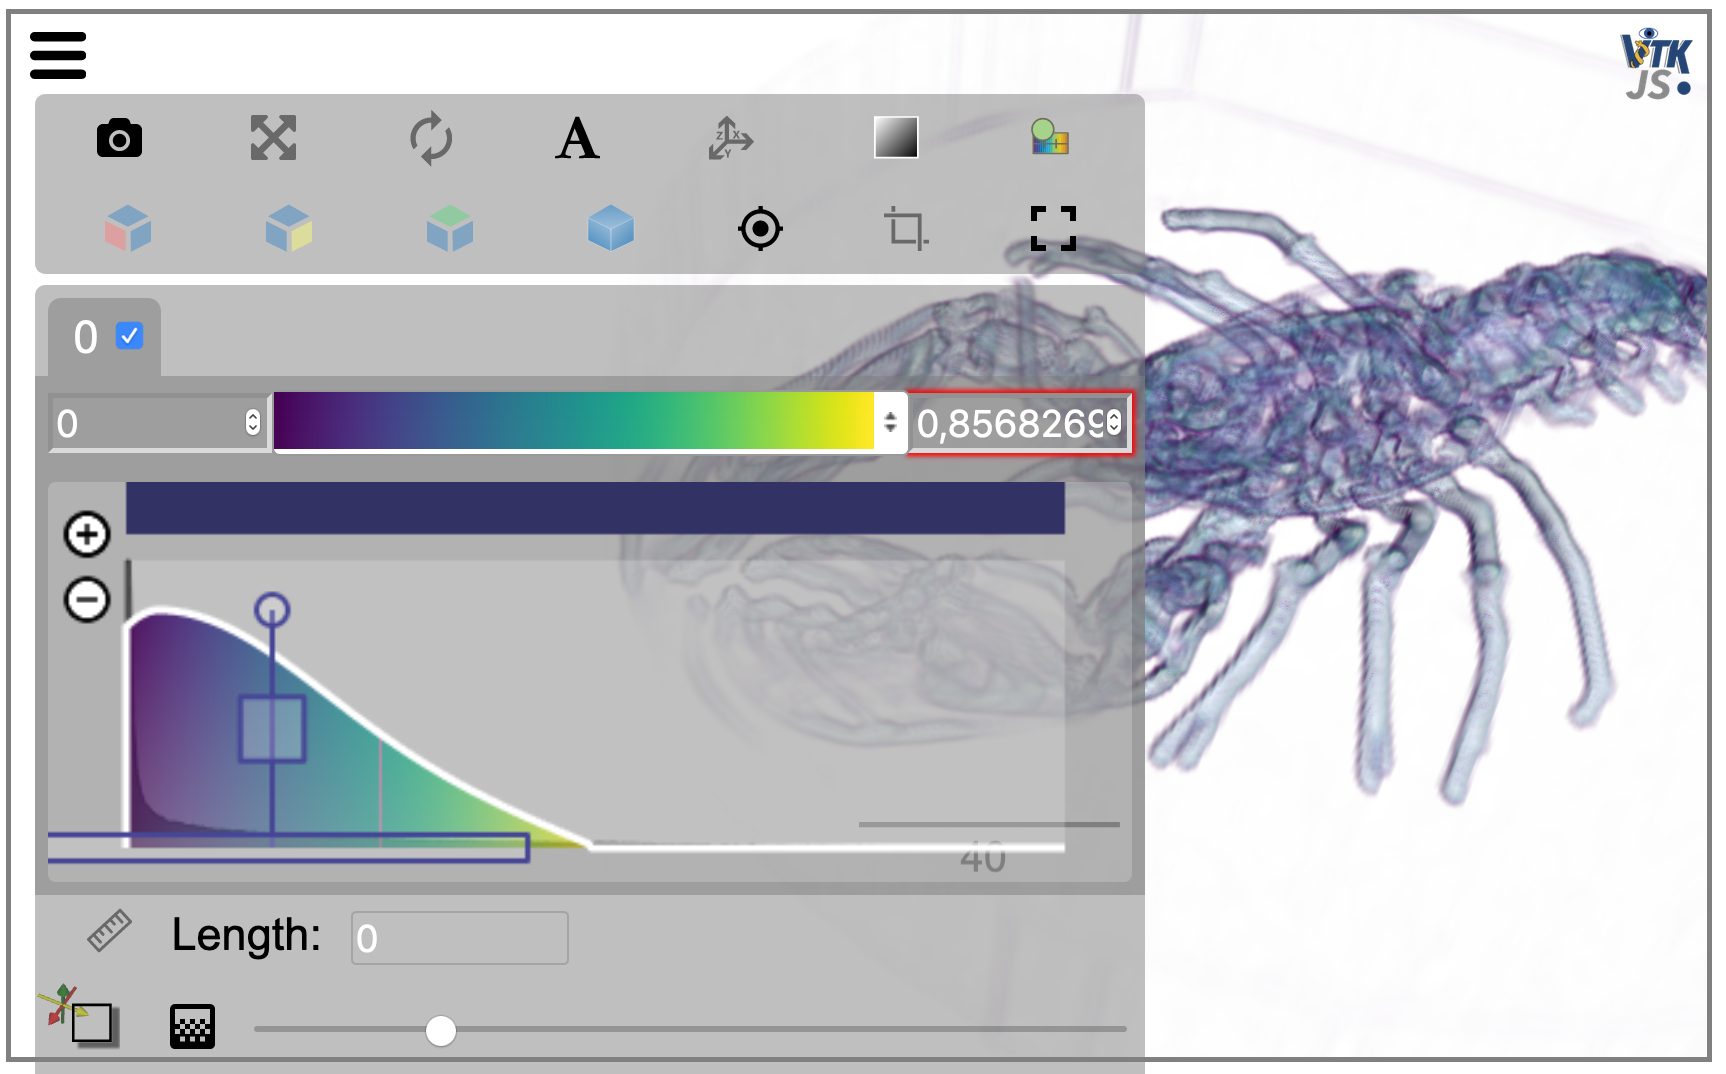
\includegraphics[width=5cm]{Images/visuDemoViewerExtract2.png}
        \caption{ }
    \end{subfigure}

  \caption{Illustration de la visualisation 3D obtenue par la démonstration. (a) Résultat d'un filtre superposé à la vérité terrrain (rouge). (b) Rehaussement effectué à partir de données fournies par l'utilisateur. (c) Réglage dynamique des couleurs et de la transparence de la fenêtre de visualisation.}
\label{Fig:Illustr3D}
\end{figure}

\subsection{Intégration aux outils Kitware}

Nous avons largement utilisé les outils de Kitware Inc. pour développer notre banc de test. L'ensemble de code repose sur la librairie ITK. Nous nous sommes aussi fortement reposés sur l'outil 3DSlicer pour la visualisation interactive des volumes 3D.

Les filtres de Jerman, Zhang, OOF et Meijering, ont été implémentés en prenant exemple sur des filtres déjà fournis par ITK (Frangi, Sato) et peuvent donc être incorporés à la libraire moyennant une vérification des conventions de nommage. De même, nous avons implémenté une interface entre les CLI (\textit{Command Line Interfaces}) des filtres et 3DSlicer. L'ensemble des filtres peut ainsi être manipulé de manière interactive dans le logiciel (Fig. \ref{fig:slicer_vesselness}).

\begin{figure}[H]
    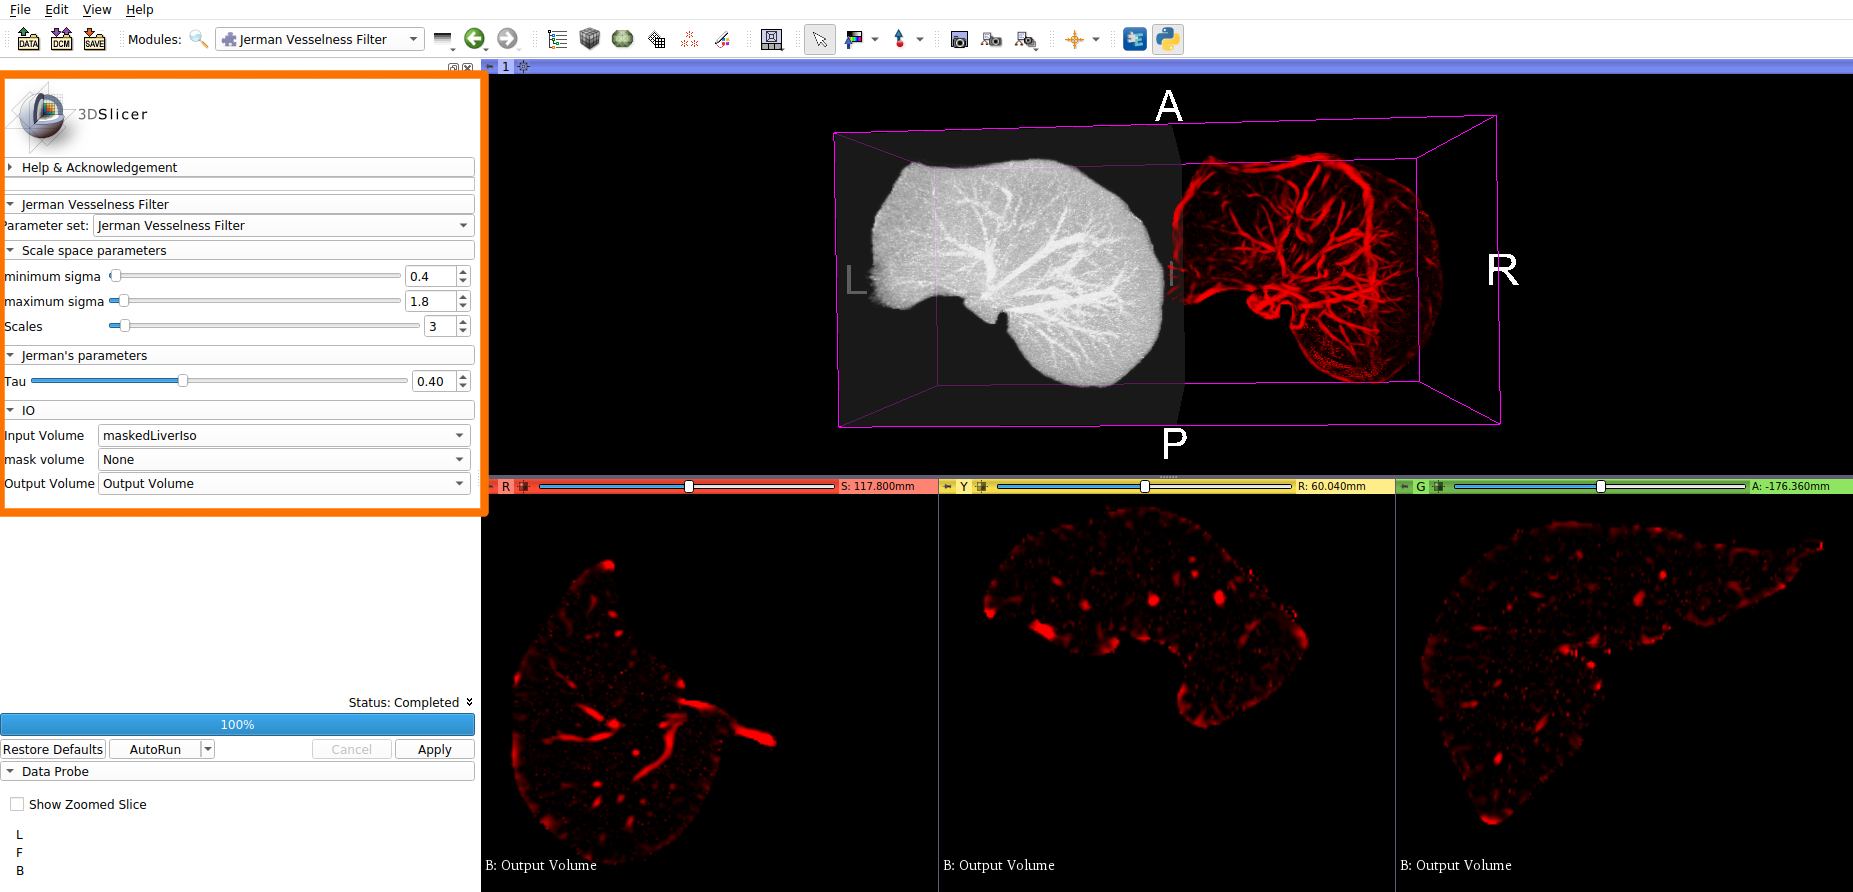
\includegraphics[height=7cm]{Images/slicer_jerman.png}
    \caption{Illustration de l'utilisation du filtre de Jerman (dont la zone des  paramètres est encadré en orange à gauche) dans 3DSlicer.}
    \label{fig:slicer_vesselness}
\end{figure}

\subsection{Plug-in d'annotation}

Nous avons aussi participé à l'élaboration d'un plug-in 3DSlicer permettant de faciliter l'annotation d'images hépatiques en 3D. L'élaboration de ce plug-in a été motivée par l'absence de jeux de données incluant des vérités terrains des vaisseaux en IRM. Ce plug-in a été développé de manière à faciliter le travail de segmentation par les médecins en fluidifiant le pipeline d'annotations.

Nous avons dans un premier temps mené une analyse des avantages et inconvénients des différents logiciels gratuits en termes de capacité et de modularité. Parmi les logiciels tels que MITK, ITK-Snap, etc. nous avons choisi 3DSlicer qui nous paraissait le logiciel le plus personnalisable, grâce à son système de plug-in et une api python ouverte.

Le Plug-In est composé de 7 onglets qui permettent :

\begin{itemize}
    \item le chargement et la gestion des images médicales
    \item la segmentation du foie ;
    \item l'annotation de la veine porte et sa segmentation ;
    \item l'annotation de la veine cave et sa segmentation ;
    \item l'annotation des tumeurs.
\end{itemize}

Les segmentations peuvent être obtenues à l'aide d'outils interactifs (tels que les croissances de région) ou en utilisant des méthodes de deep learning. 
Le plug-in permet l'annotation de la ligne centrale des vaisseaux en apposant des nœuds aux embranchements des vaisseaux. Le positionnement des points est accompagné d'une nomenclature dynamique permettant de nommer les différentes branches. A partir de ces points, le plug-in permet d'initialiser une segmentation voxélique effectuée automatiquement par le module VMTK (Vascular Modeling Tool Kit). L'utilisateur peut ensuite raffiner manuellement la segmentation (Fig. \ref{fig:slicer_plug_in}).

\begin{figure}[H]
    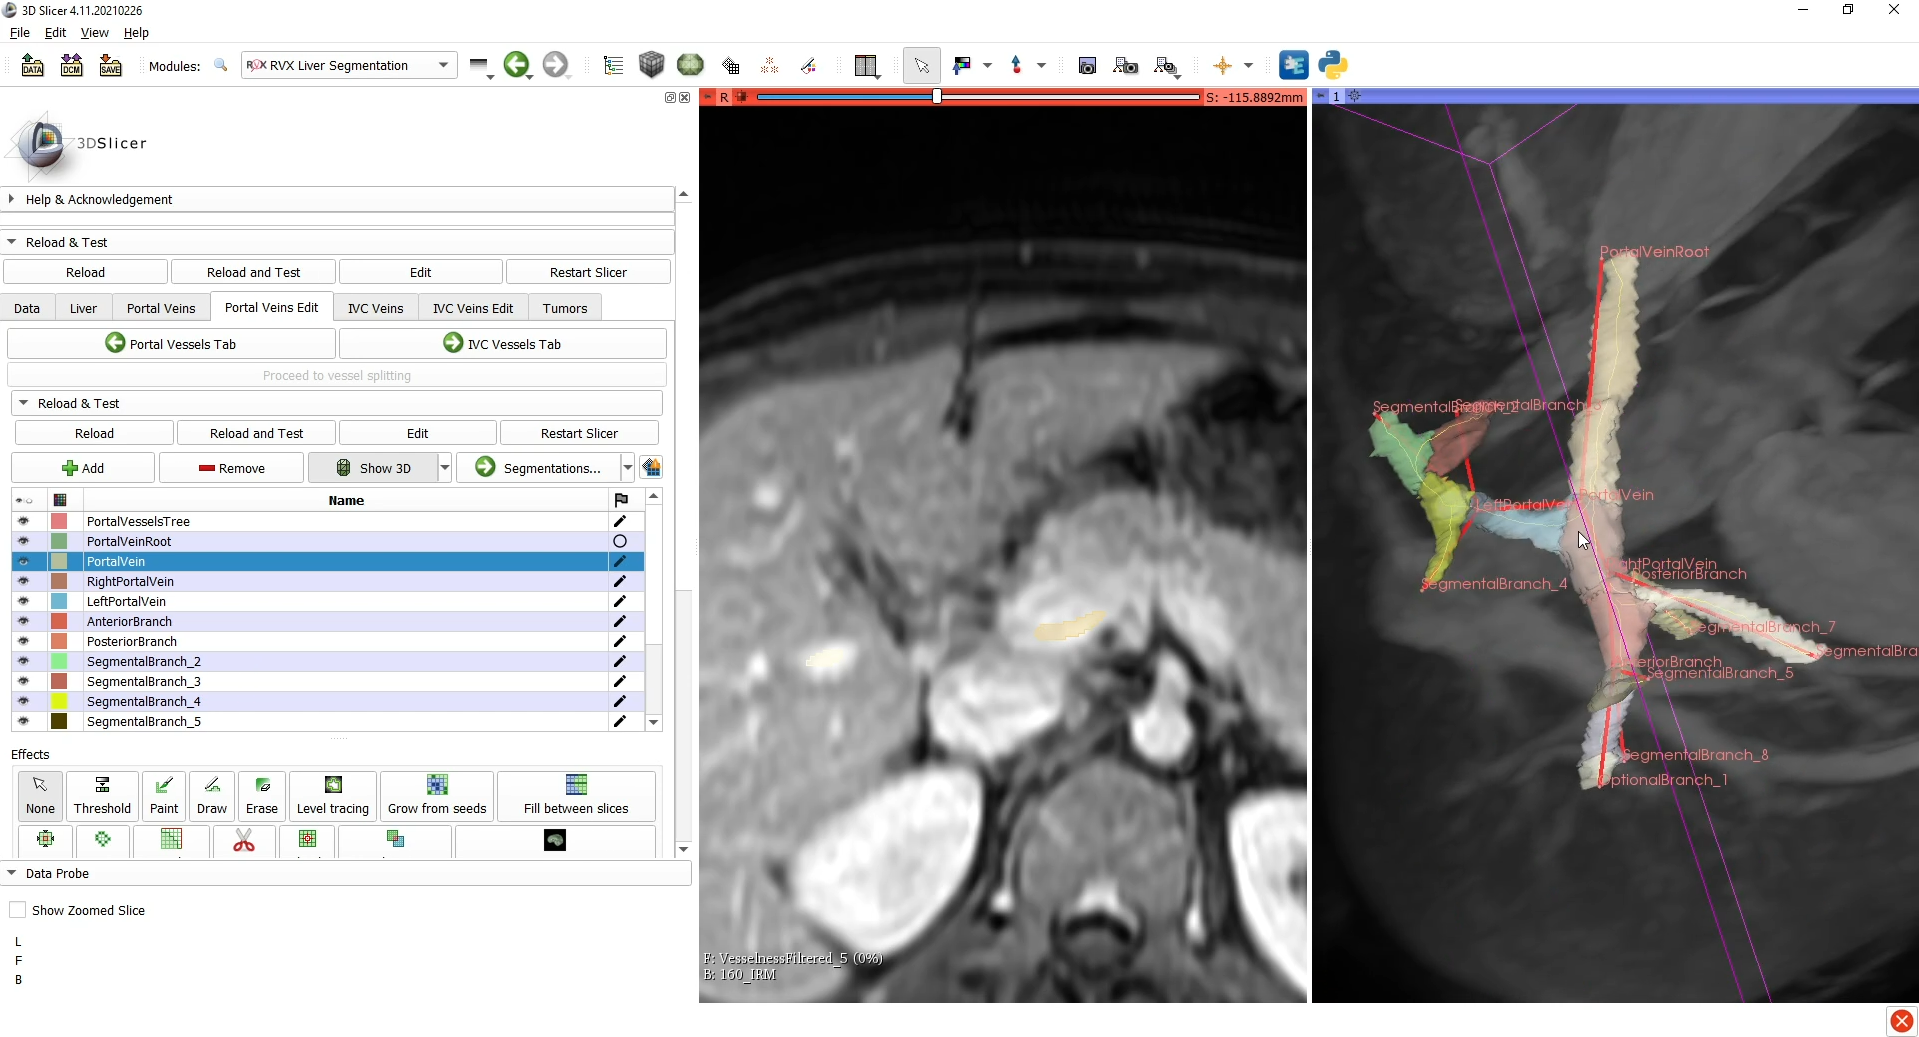
\includegraphics[height=7cm]{Images/plug_in_segmentation.png}
    \caption{Segmentation et classification des vaisseaux en utilisant le Plug-In R-Vessel-X.}
    \label{fig:slicer_plug_in}
\end{figure}

L'ensemble des segmentations peut être exporté sous forme de volumes binaires ainsi que le graphe des lignes centrales des vaisseaux sous la forme de fichier csv contenant les points et une matrice d'adjacence.
Ce plug-in a fait l'objet d'une publication dans le journal JOSS (Journal of Open Source Software) \cite{Lamy2022_JOSS} ainsi qu'aux conférences VPH 2020 \cite{Lamy2020_VPH_plugin} et EASL 2022 (Liver Cancer Summit) \cite{Lamy2022_EASL}.




